\section{Formulación del problema}
\label{sec:problem}

El desafío presentado se basa en una situación real relacionada con una empresa que gestiona un elevado volumen de pedidos de cajas de diferentes tipos. Cada semana, la empresa busca determinar cuántas cajas de cada tipo debe enviar en un contenedor para maximizar el beneficio total de dicho envío.

El desafío principal al que se enfrenta la empresa es optimizar el proceso de envío de cajas, donde cada una proporciona un ingreso específico. El objetivo es maximizar el uso del espacio en los contenedores para obtener el mayor beneficio posible. Dado que las cajas tienen distintos tamaños, pesos y valores, se plantea una dificultad para estimar de manera eficaz cómo llenar completamente un contenedor sin desperdiciar espacio. Este desperdicio no solo implica una pérdida financiera, sino que también tiene un impacto ambiental negativo, ya que cada viaje consume combustible y genera emisiones contaminantes.

Para abordar este desafío, es crucial considerar el proceso manual de carga del contenedor. El procedimiento actual de carga no está optimizado y no considera la disposición óptima de las cajas, lo que lleva a una carga subóptima y un desperdicio de espacio. Por tanto, es necesario revisar y mejorar este procedimiento para asegurar que se aproveche al máximo el espacio disponible en los contenedores.

El procedimiento de carga manual debe ser meticulosamente evaluado y optimizado. Este aspecto es crucial porque los operarios son los responsables de organizar físicamente las cajas en el contenedor. Un procedimiento manual de carga bien diseñado garantizaría que se aproveche cada centímetro disponible del contenedor, reduciendo así el espacio vacío y aumentando la rentabilidad del envío.

Respecto a las restricciones que se generan debido a la carga manual, se consideran las siguientes:

Los paquetes que son cajas de forma rectangular, pueden variar en tamaño, peso y valor, pero han sido concebidos previamente para que puedan ser cargados manualmente es decir que no son paquetes muy grandes o pesados.

Los paquetes que comparten el mismo tamaño, peso y valor estrictamente se consideran del mismo tipo, dos paquetes pueden tener el mismo tamaño y peso pero distinto valor, lo que los convierte en tipos diferentes. El valor de un paquete no depende de su tamaño o peso, es decir que un paquete sea más grande y pesado que otro no implica que sea de mayor valor y viceversa.

Los paquetes llegan a la puerta del contenedor agrupados por tipo y en un orden específico, los paquetes pueden apilarse unos sobre otros independientemente de su tipo ya que las cajas lo soportan y sus pesos no son muy disparejos, pero se debe asegurar la estabilidad de la carga. Por ejemplo en el la Figura \ref{fig:paquetes_apilados} se muestra un ejemplo de cómo se apila un tipo de paquete encima de otro.

\begin{figure}[H]
    \centering
    \includesvg[width=0.5\textwidth]{Figures/paquetes_apilados}
    \caption{Ejemplo de cómo se apila un tipo de paquete encima de otro.}
    \label{fig:paquetes_apilados}
\end{figure}

Para asegurar la estabilidad de la carga, por ejemplo un paquete más grande no puede estar encima de uno más pequeño, es decir un paquete siempre debe tener una base sobre la que se apoye, en la Figura \ref{fig:paquetes_mal_apilados} se muestra un ejemplo de una carga inestable.

\begin{figure}[H]
    \centering
    \includesvg[width=0.5\textwidth]{Figures/paquetes_mal_apilados}
    \caption{Ejemplo de una carga inestable.}
    \label{fig:paquetes_mal_apilados}
\end{figure}

Para facilitar la carga manual se considera de que todos los paquetes de un mismo tipo deben mantener la misma orientación, es decir que no se pueden colocar paquetes de un mismo tipo en diferentes orientaciones, por ejemplo en la Figura \ref{fig:paquetes_mal_orientados} se muestra un ejemplo de cómo no se deben colocar los paquetes, ya que dificultaría al operario seguir dicho procedimiento, además que aumentaría el riesgo de desperdiciar espacio o de que la carga sea inestable.

\begin{figure}[H]
    \centering
    \includesvg[width=0.5\textwidth]{Figures/paquetes_mal_orientados}
    \caption{Ejemplo de cómo los paquetes de un mismo tipo tienen distinta orientación.}
    \label{fig:paquetes_mal_orientados}
\end{figure}

Muchas de las cajas están diseñadas para ser apiladas y soportar un gran peso encima siempre y cuando se respete la indicación de mantener una posición mirando hacia arriba, por lo que los paquetes solo pueden ser girados en un eje, por ejemplo en la Figura \ref{fig:paquetes_girados} se muestra un mismo tipo de paquete girado en un eje.

\begin{figure}[H]
    \centering
    \includesvg[width=0.5\textwidth]{Figures/paquetes_girados.svg}
    \caption{Ejemplo de cómo los paquetes de un mismo tipo pueden ser girados en un eje.}
    \label{fig:paquetes_girados}
\end{figure}

Para evitar la fatiga del operador de levantar los paquetes, la empresa suele usar cintas o bandas transportadoras, para aprovechar su uso, esto implica que los paquetes deben ser colocados en primer lugar lo más profundo posible del contenedor, es decir que los paquetes que están siendo cargados, deben ser colocados en la parte más alejada de la puerta del contenedor, de este modo también se evita que los paquetes obstruyan el ingreso del personal de carga al contenedor. En la Figura \ref{fig:cinta_transportadora} se muestra un ejemplo de cómo se puede hacer uso de una cinta transportadora que desliza los paquetes hacia el fondo del contenedor, mientras el contenedor se va llenando la cinta se va moviendo en sentido contrario.

\begin{figure}[H]
    \centering
    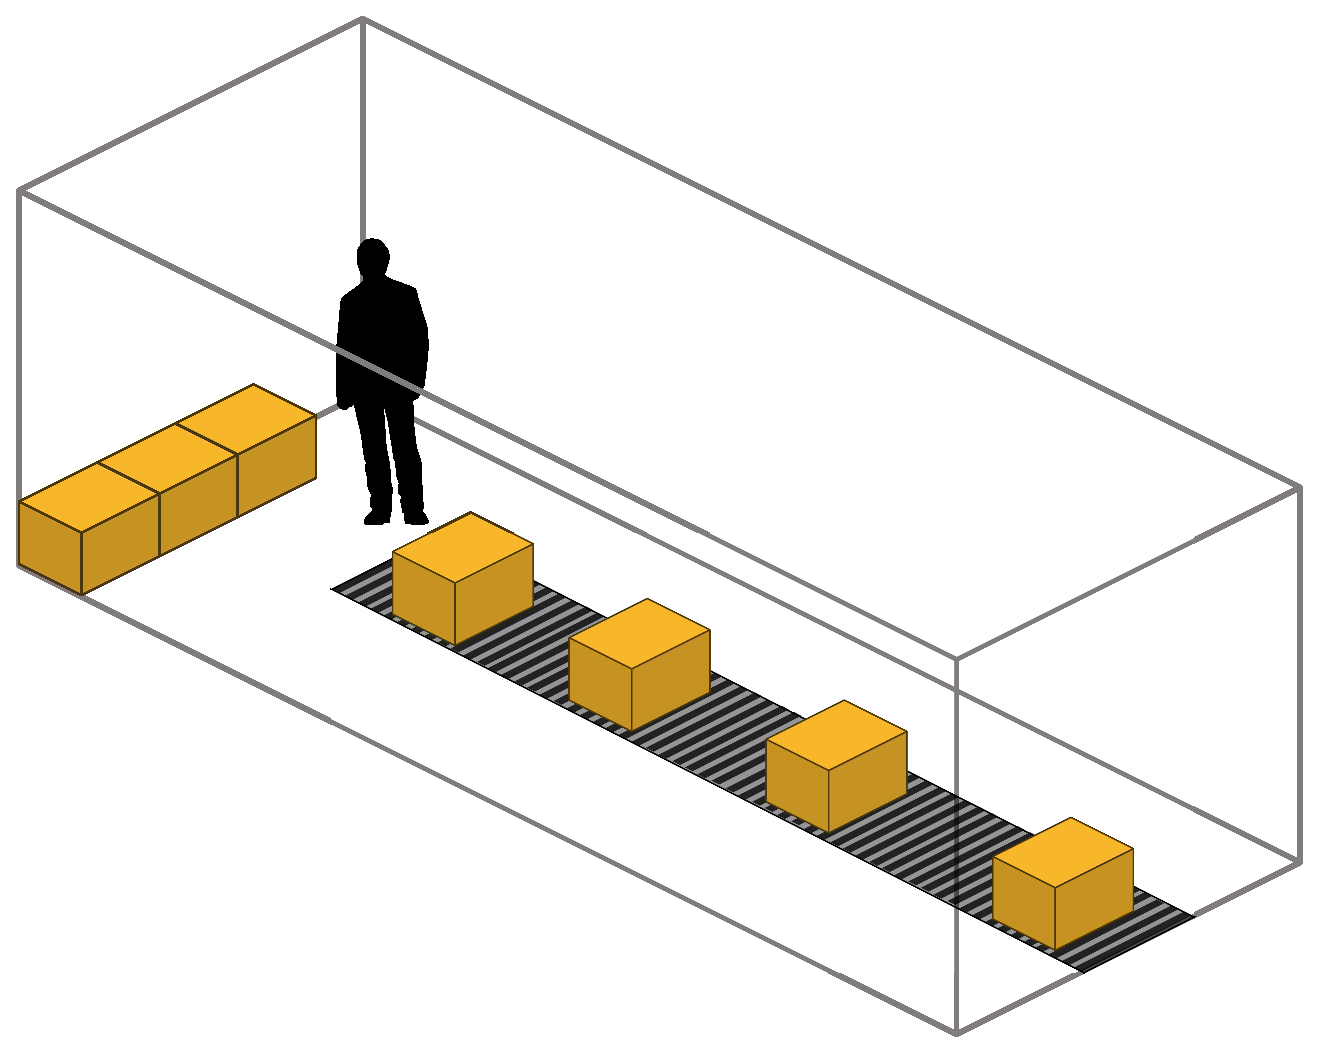
\includegraphics[width=0.5\textwidth]{Figures/cinta_transportadora.eps}
    \caption{Ejemplo del uso de una cinta transportadora.}
    \label{fig:cinta_transportadora}
\end{figure}

La empresa ha implementado un procedimiento específico para guiar a los operadores en la colocación de paquetes dentro del contenedor, con el objetivo de cumplir con todas las condiciones preestablecidas. No obstante, este procedimiento aún no está optimizado y no garantiza la disposición óptima de los paquetes, lo que conduce a una carga subóptima y al desperdicio de espacio.

El desafío que se enfrenta es conocer con anticipación la cantidad de paquetes por tipo que deben cargarse en el contenedor, así como definir el orden de carga y la rotación de cada tipo de paquete. El objetivo es lograr una disposición que no solo cumpla con las restricciones de espacio y los requerimientos del llenado manual, sino que también maximice el valor económico de la carga transportada y la eficiencia en el uso del espacio .

\subsection{Definición formal del problema}

El problema de la carga manual de paquetes en un contenedor se define formalmente de la siguiente manera:

\begin{figure}[H]
    \centering
    \includesvg[width=0.5\textwidth]{Figures/container.svg}
    \caption{Contenedor con dimensiones $W$, $L$, $H$}
    \label{fig:container}
\end{figure}

Siendo un contenedor una caja de forma rectangular, de ancho $W$, largo $L$, alto $H$, en la figura \ref{fig:container} se muestra un contenedor con sus dimensiones, y una capacidad de carga $P$, se tiene definido unos tipos de paquetes también de formas rectangulares $t \in T = \{0, 1, 2, \ldots, n\}$, donde cada tipo $t$ posee ciertas dimensiones de ancho $w_t$, largo $l_t$, alto $h_t$, también posee un peso $p_t$ y un valor $v_t$, además se conoce la cantidad máxima $q^{max}_t$ de paquetes que dispone la empresa por cada tipo.

En este problema, consideramos que $W$, $L$, $H$ y $P$ , $w_t$, $l_t$, $h_t$, $p_t$, $q^{max}_t$ son enteros positivos, los cuales podrían ser representados en unidades de medida centímetros, milímetros, kilogramos, litros, entre otros.

\begin{figure}[H]
    \centering
    \includesvg[width=0.5\textwidth]{Figures/rotacion.svg}
    \caption{Rotación de un paquete en el eje $x$}
    \label{fig:rotation}
\end{figure}

Se tienen restricciones de rotación debido al enfoque de carga manual, en el cual se establece que $\forall r \in r_t, r \in \{0, 1\}, t \in T$ donde $0$ representa que el tipo no se encuentra girado y $1$ que el tipo está girado 90 grados en el eje $x$, esto se puede ver en la figura \ref{fig:rotation} a) sin rotación y b) con rotación. Esto implica que los anchos y largos pueden intercambiarse, mientras que la altura no puede ser modificada.

Por otro lado para facilitar la carga manual, se debe disponer de un orden de carga $o_t$ para cada tipo $t$, donde $o_t \in O = \{0, 1, 2, \ldots, n\}$, que indica el orden en el que se debe cargar cada tipo de paquete en el contenedor.

El problema consiste en determinar la cantidad de paquetes por cada tipo a cargar $\tilde{q}_t$ (la cual se encuentra en torno a la cantidad máxima por tipo, $0 \leq \tilde{q}_t \leq q^{max}_t$) y el orden de carga de cada tipo $o_t$ con determinada rotación $r_t$, de tal modo que se pueda obtener la disposición óptima de los paquetes en el contenedor, asegurando el cumplimiento de las restricciones relacionadas al espacio disponible. Además, se busca maximizar en primer lugar el costo total de la carga ($\max \sum_{t \in T} v_t \cdot \tilde{q}_t$) y en segundo lugar maximizar la utilización del espacio del contenedor ($\max \sum_{t \in T} w_t \cdot l_t \cdot h_t \cdot \tilde{q}_t$).


\subsection{Procedimiento de carga manual}

Para estandarizar la carga manual y facilitar el modelado por ordenador, así como simplificar la labor del operador, se han establecido una serie de supuestos, restricciones y normas que deben seguirse para optimizar la carga de paquetes en el contenedor.

En relación con la definición del problema, se establecen las siguientes suposiciones acerca de los paquetes:

\begin{itemize}
    \item Los paquetes son cajas de forma rectangular.
    \item Los paquetes pueden variar en tamaño, peso y valor.
    \item Los paquetes presentan tamaños y pesos razonables para ser cargados manualmente.
    \item Los paquetes que comparten el mismo tamaño, peso y valor estrictamente se consideran del mismo tipo.
    \item Dos paquetes pueden tener el mismo tamaño y peso pero distinto valor, lo que los convierte en tipos diferentes.
    \item El valor de un paquete no depende de su tamaño o peso, es decir que un paquete sea más grande y pesado que otro no implica que sea de mayor valor y viceversa.
    \item Los paquetes llegan al contenedor agrupados por tipo y en un orden específico.
    \item Los paquetes pueden apilarse unos sobre otros, independientemente de su tipo, pero se debe asegurar la estabilidad de la carga.
    \item Cada tipo de paquete tiene una cantidad fija deseada que debe ser cargada en el contenedor.
    \item Todos los paquetes de un mismo tipo deben mantener la misma orientación.
    \item Los grupos de paquetes llegan en bloques del mismo tipo o de forma secuencial, por ejemplo, a través de cintas transportadoras.
\end{itemize}

Las suposiciones relacionadas con el operario son las siguientes:

\begin{itemize}
    \item Uno o varios operarios realizan la carga de los paquetes en el contenedor de forma manual.
    \item El operario recibe indicaciones previas sobre cómo cargar los paquetes en el contenedor, incluyendo el orden, la cantidad y la orientación de cada tipo de paquete.
    \item Las indicaciones también podrían especificar los espacios que deberán quedar vacíos en el contenedor, los cuales pueden ser llenados con material de relleno para evitar que los paquetes se muevan durante el transporte.
    \item Las indicaciones previas proporcionadas al operario son el resultado de la solución del problema de optimización de la carga.
    \item El objetivo del operario es seguir las indicaciones previas de manera eficiente y precisa, sin necesidad de tomar decisiones adicionales sobre la disposición de los paquetes.
\end{itemize}

El procedimiento de carga manual se basa en la combinación de las suposiciones, restricciones y reglas mencionadas anteriormente, con el objetivo de lograr una carga eficiente y organizada de los paquetes en el contenedor. Este procedimiento se implementa siguiendo una metodología específica que guía al operario en la colocación de los paquetes, asegurando que se cumplan todas las condiciones establecidas.

En el siguiente capítulo se presentará un algoritmo metaheurístico para resolver el problema de optimización de la carga manual de paquetes en un contenedor, considerando las restricciones de espacio del contenedor, así como las restricciones de rotación y orientación de los paquetes.
